\noindent Nowadays, information is stored digitally and can be easily accessed at any time. Most people are connected continuously with numerous devices through Internet, an increasingly safe platform due to the work of many specialists, but in which cybercriminals still find vulnerabilities and attack all kinds of entities to acquire profits \cite{STDWNCRY}. There are many malicious programs such as viruses, worms or trojans that can damage systems. One of the most common cyberattacks according to a report published by the Europol (European Union Agency for Law Enforcement Cooperation) \cite{ZETTER} is ransomware. Ransomware is a malware type that blocks devices or prevents data access using private key encryption until the victims pays an economic ransom, usually in bitcoin. Data theft extortion has been used since 2005, but due to the rise of ransomware and bitcoin, the number of cases has increased hugely and almost 40\% of companies have suffered at least one ransomware attack according to a study by Malwarebytes \cite{2}, which shows the evidence that these malicious programs are an important threat to detect and mitigate as soon as possible.

Cybercriminals are becoming more creative and innovative and the damage caused by them is getting worse. Figure \ref{fig:im0} shows the prediction of mitigating damage cost against ransomware attacks for the year 2021, making it clear that there has been a huge increase in comparison to the past decade. These costs are both to the investment in defending systems and the losses resulting from not being able to use the devices and the ransom payments.

\begin{figure}[h!]
\begin{center}
{\scalebox{.68}{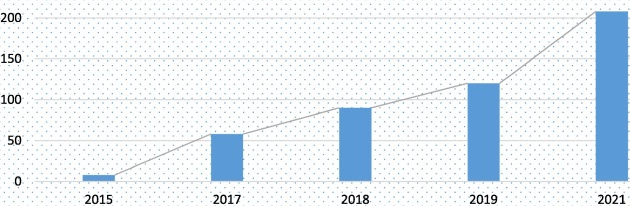
\includegraphics{images/grafica11.png}}}
\end{center}
\caption{Ransomware cost prediction in billions of dollars}
\label{fig:im0}
\end{figure}

Figure \ref{fig:cove} shows the results obtained from a Coveware study \cite{4} about most attacked industries by ransomware attacks in the last quarter of 2020. Professional services, public sector and health sector are the most affected, considering that they are the most profitable for criminals. This is caused by the need of being in constant operation and because they store sensitive data, so they usually pay the ransom to recover their data and the access to the system as soon as possible.

\begin{figure}[h!]
\begin{center}
{\scalebox{.19}{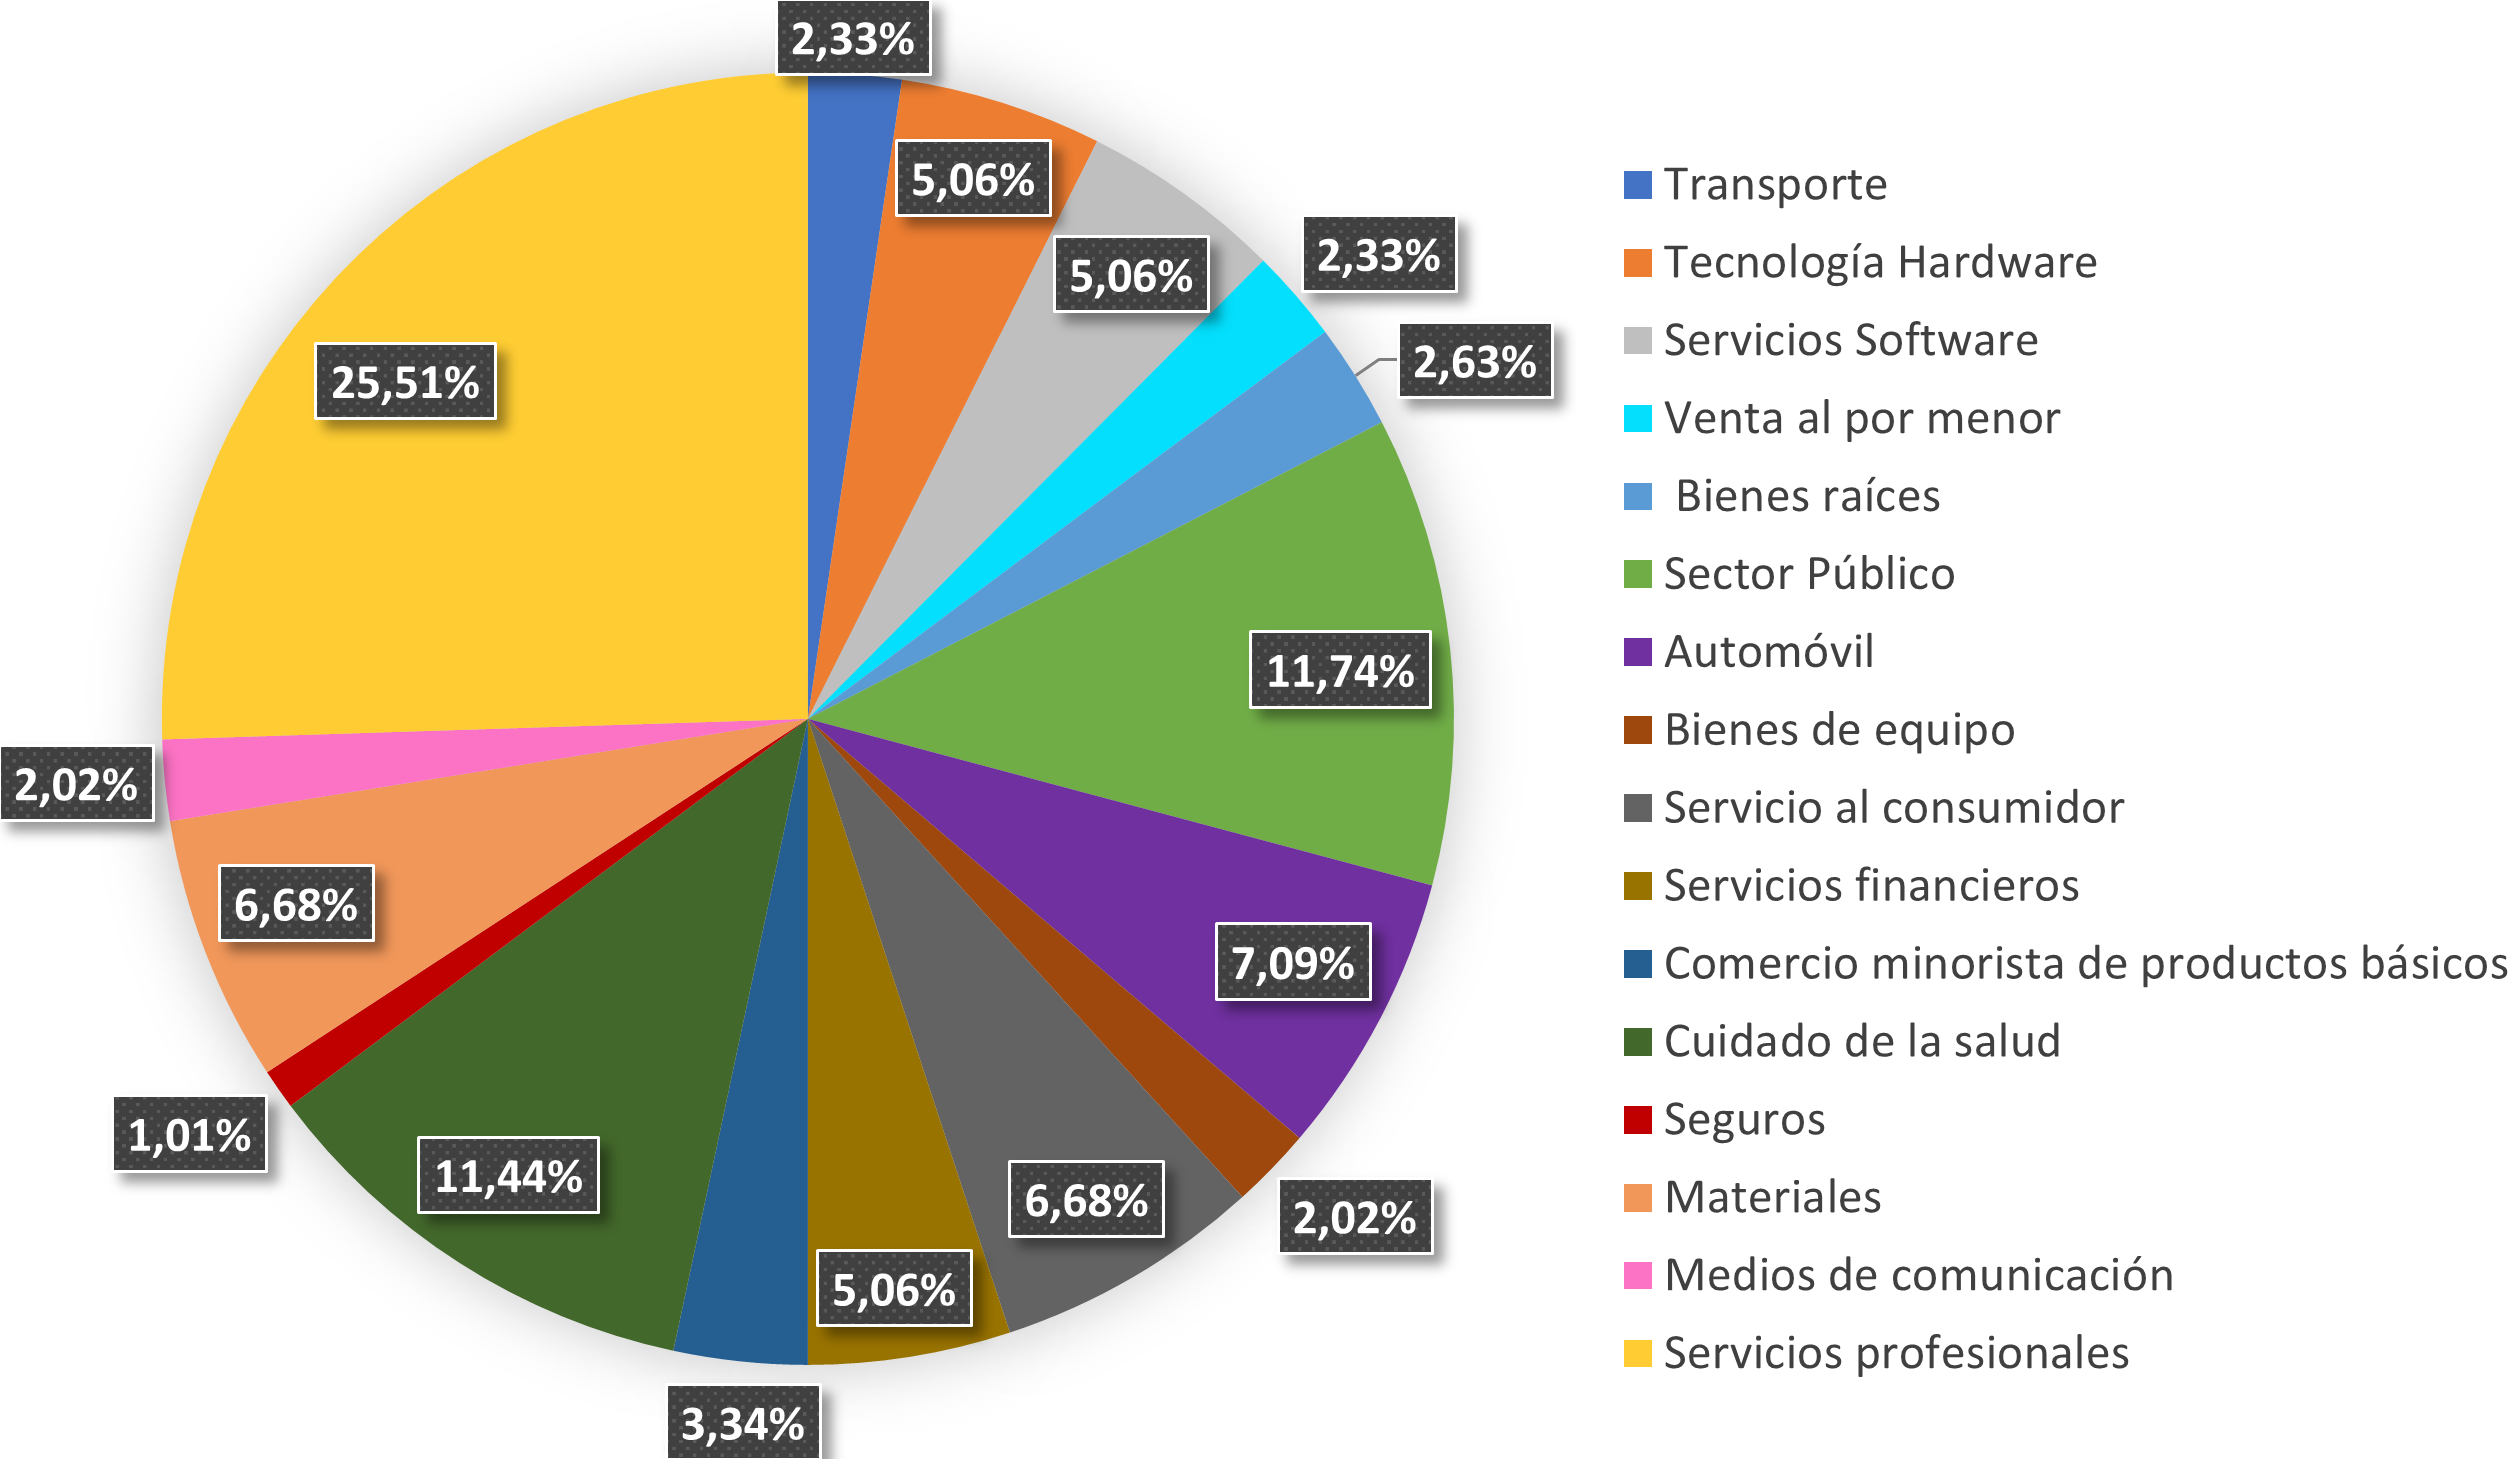
\includegraphics{images/industries2.png}}}
\end{center}
\caption{Most attacked sector by ransomware in the third quarter of 2020}
\label{fig:cove}
\end{figure}

The risk of this is just as significant for large enterprises as for \gls{SME}. These companies also use, produce and store large amounts of data. The difference is that smaller companies have to deal with these problems using limited resources. Therefore, they need an economic effort to draw up security strategies against these cyberattacks \cite{KURPJUHN20155}.

The current health situation is also added to the suggested scene, a pandemic caused by the \gls{COVID-19} disease. While this disease was spreading around the world, a technological threat was growing based on indiscriminate cyberattacks and cybercampaigns focused on public authorities and organisations \cite{LALLIE2021102248}, as well as on people based on their misinformation and concern, such as the false distribution of \gls{COVID-19} books \cite{MALWLABS}, the fraudulent medicine offered via email \cite{NORTON}, etc. Another factor that supported the increase of cyberattacks, especially ransomware attacks, is the establishment of remote work. In Spain, these attacks increased by 160\% in the second half of 2020, leading the European ranking, due to the fact that companies that focused their efforts on establishing remote work environments, did not apply the necessary security to do so \cite{ELPAIS}. In Spain, the affected companies have not been only private ones, public institutions have as well received ransomware attacks. The \gls{SEPE} had to paralyse its services for 5 days, adding 20 without remote work due to an attack in March 2021 by Ryuk ransomware, causing a serious situation, so the \gls{SEPE} activity shot up due to the pandemic impact on unemployment \cite{RYUKSEPE}.

The development of technology provides benefits and facilities in all fields and tasks, even in the more quotidian. An example of this is \gls{IoT}, that is defined as the integration of real life places and objects that use Internet through an interconnected network of devices, sensors, software, etc. that store and exchange data \cite{IoTDEF}. However, the existence of this technology allows for the number of ransomware attacks to grow over time, especially after the use of intelligent \gls{IoT} devices, in particular smartphones. In Figure \ref{fig:im1} we can observe the amount of ransomware attacks intended to smartphones in each quarter of 2018. Figure \ref{fig:im2} shows a prediction of how the use of these devices will rise due to the growth of \gls{IoT}. Based on this data we can predict that the amount of attacks will continue rising and it demonstrates the need both for protecting users and organisations from this type of attacks and for providing users and workers the existing information to act in a responsible and safe way to prevent them \cite{HUMAYUN2021105}.

% IMAGEN 1
\begin{figure}[htb]
\begin{center}
{\scalebox{.4}{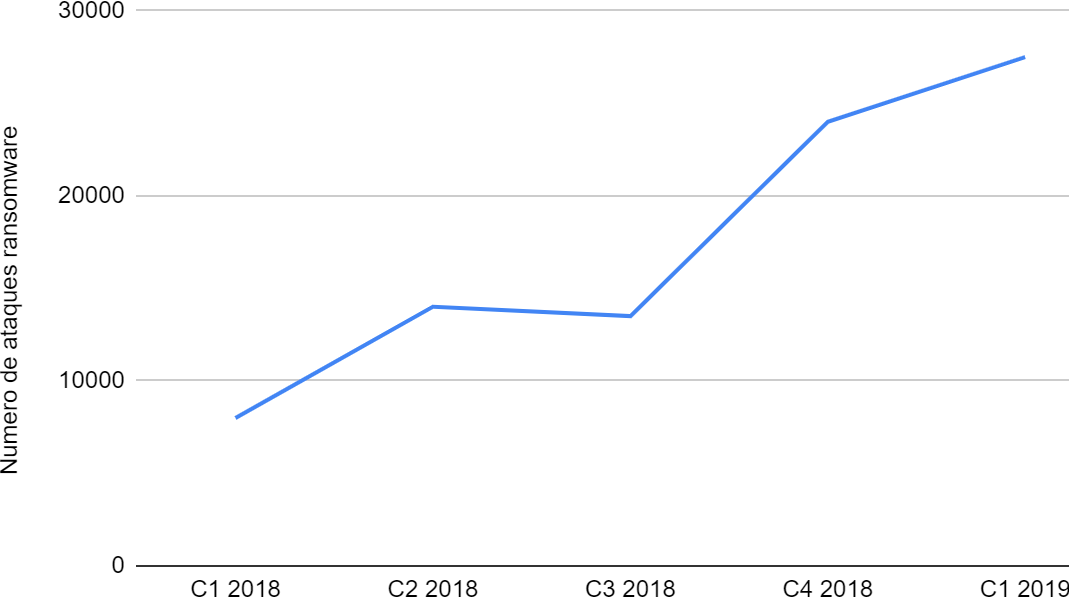
\includegraphics{images/grafica4.png}}}
\end{center}
\caption{Ransomware attacks on mobile devices}
\label{fig:im1}
\end{figure}


% IMAGEN 2
\begin{figure}[htb]
\begin{center}
{\scalebox{.6}{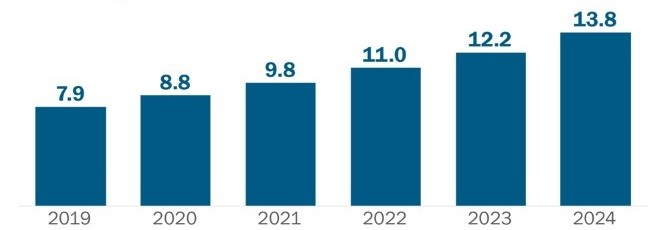
\includegraphics{images/grafica31.jpg}}}
\end{center}
\caption{Prediction of the number of mobile IoT devices in billions}
\label{fig:im2}
\end{figure}


\section{Motivation}
\noindent As seen in Section \ref{intro}, the impact of the ransomware attacks on companies in recent years is evident, causing large financial investments from those companies to improve their security.
\gls{SME}s have greater difficulty in meeting those expenses due to the lack of prevention systems, specialists focused on cybersecurity and information related to this sector, therefore they are more exposed to the attacks.


In the European Union, \gls{SME} are a fundamental pillar of the economy, representing in September 2020 an astonishing 99,8\% of all employing companies, 65\% of private sector employment and 54\% of the private sector. They have also suffered large economic losses and an even larger number of closures \cite{NBER} due to the \gls{COVID-19} pandemic.
Due to all of those factors, the main motivation for this study is the development of a ransomware detection model that meets the following requirements: High precision, reliability, scalability, easy to use, speed and open source software.


With this approach it is possible to carry out a prevention strategy against ransomware attacks and mitigate the impact of the damage caused by them, drastically reducing the expenses of the \gls{SME}.


%\section{Context}
%\noindent This Final Degree Project has been carried out within the Analysis, Security and Systems Group (GASS Group \cite {GASS01}, \url{https://gass.ucm.es/}, Group 910623 from the catalogue of groups recognised by the \gls{UCM}) as part of a research project approved by the European Commission.


\section{Objectives}
\noindent At the beginning of this work, a series of objectives and guidelines were established to ensure its quality and correct development:
\begin{itemize}
    \item Use the acquired skills during the academic degree.
    \item Develop a \gls{ML} model capable of identifying ransomware samples with great precision.
    \item Create a large enough dataset to guarantee the reliability of the obtained results.
    \item Develop and deploy a laboratory to analyse the malware samples.
    \item Prove the effectiveness of the Windows \gls{API} calls done by an executable as a ransomware detection mechanism.
\end{itemize}


\section{Work Plan}
\noindent The development of this work has been carried out in the following phases:
\begin{enumerate}
    \item \textbf{Research}: This phase was carried out during the first four months to acquire the necessary information for the development of the work. At the beginning of this phase, several meetings were held where the objectives of the project and the necessary knowledge were explained, which was the fundamental concepts of machine learning. The main research tool used was \textit{Google Scholar}, since it allows to search for scientific articles with ease and facilitates the citing. Articles and papers on detection of both ransomware and malware were searched, as well as books on malware analysis to gain a deeper understanding of the topic and the context of the study.
    \item \textbf{Development}: The development of the model began once the necessary knowledge has been obtained. The investigation was not completely abandoned, but it was second priority. During this phase, the necessary data was obtained and the two \textit{datasets} were built to train and evaluate the proposed model. For coding the model and implementing the \gls{ML} algorithms, the programming language Python and the \textit{scikit-learn} library were used. 
    \item \textbf{Experimentation and results}: In this phase the developed model with the extracted data was experimented on. It was necessary to evaluate the results obtained and to demonstrate the validity of the model, so the K-fold cross validation was used. The experimentation was vital for the development phase, since the model had to be modified to improve the results. The parameters were adjusted, more data was obtained...
    \item \textbf{Documentation}: This phase was carried out in parallel to the rest of the phases. It started in the final months of the research phase and continued throughout the development and experimentation phases. All the members of the team participated in the writing of the documentation, working together in all of the sections. Any update had to be accepted and reviewed by the other team members.
\end{enumerate}

The model developed in this work was uploaded to the  Gitlab repository \href{https://gitlab.fdi.ucm.es/marina.lopez/tfg-ransomware-20-21}{TFG Ransomware 20-21}

Figure \ref{fig:gantt} is a Gantt chart where the different activities performed by the team throughout the months and their duration is shown.

\begin{figure}[htb]
\begin{center}
{\scalebox{.9}{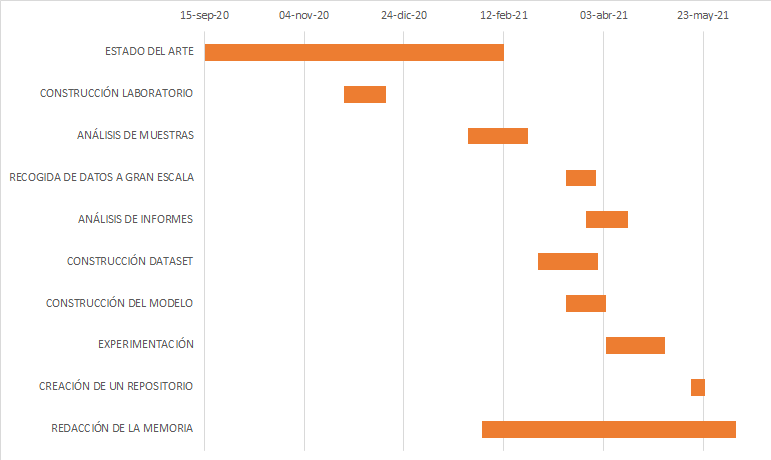
\includegraphics{images/gant.png}}}
\end{center}
\caption{Gantt chart of the performed tasks.}
\label{fig:gantt}
\end{figure}

\section{Work Structure}
\noindent The rest of the work is organised in 10 chapters, following this structure:

Chapter \ref{Capitulo2} introduces ransomware, explaining the fundamental concepts about malware and the different types, the business model that cybercriminals follow to profit from the attacks and the historical evolution of ransomware, detailing the different attacks that happened in the world each year. The different types of ransomware, the families, the most common spreading methods and subsequently the mode of operation to infect the victim's system are also explained. The chapter ends with the explanation of techniques used by antivirus programs to recognise the presence of ransomware, and with some prevention strategies and actions that every company should follow to protect their systems from these attacks, and if they are a victim of them, what steps they should follow to recover their data.

Chapter \ref{Capitulo3} addresses the types of malware analysis that exist and the limitations of each one, the tools used for the analysis and the different identification techniques. Machine learning applied to malware analysis is also discussed, exposing how a model is built using Python as a programming language and the different algorithms that exist. The supervised learning algorithms are the main focus since they are most commonly used in malware and ransomware detection and analysis.

Chapter \ref{Capitulo4} shows related works to the topic of malware and ransomware analysis and detection using \gls{ML} models and algorithms. A distinction is made between papers that only analyse malware from those that analyse ransomware, and within the ransomware works, those that use Windows \gls{API} calls to build their models are distinguished from those that do not.

Chapter \ref{Capitulo5} explains the technologies used to develop the proposed \gls{ML} model, the sandbox environment and the process of obtaining the data. The flow diagram of the proposed system is shown and the development of the analysis laboratory for the study of ransomware and goodware samples is discussed, from which the calls to the Windows \gls{API} are extracted for the construction of the datasets. The data is then cleaned to discard those elements that are not relevant for the study. Finally, it is explained how the model will be created.

Chapter \ref{Capitulo6} discusses the experiments performed and the metrics used to demonstrate the effectiveness of the model to detect ransomware. After doing the experiments on the two datasets and showing the parameters used for their development, the final results are obtained and validated with K-fold cross validation. The algorithm that performs better than others is chosen and the results obtained with it are compared with the results of the related works presented in Chapter \ref{Capitulo4}.

Chapter \ref{Capitulo7} shows the conclusions of the work after analysing the results, and exposes future lines of research.

Chapter \ref{Capitulo8} explains the individual contributions of each team member to the development of the work.

Chapters \ref{Capitulo9} and \ref{Capitulo10} are the English translations of Chapters \ref{Capitulo1} and \ref{Capitulo7}.